\FloatBarrier
\begin{figure}[!h]
\centering
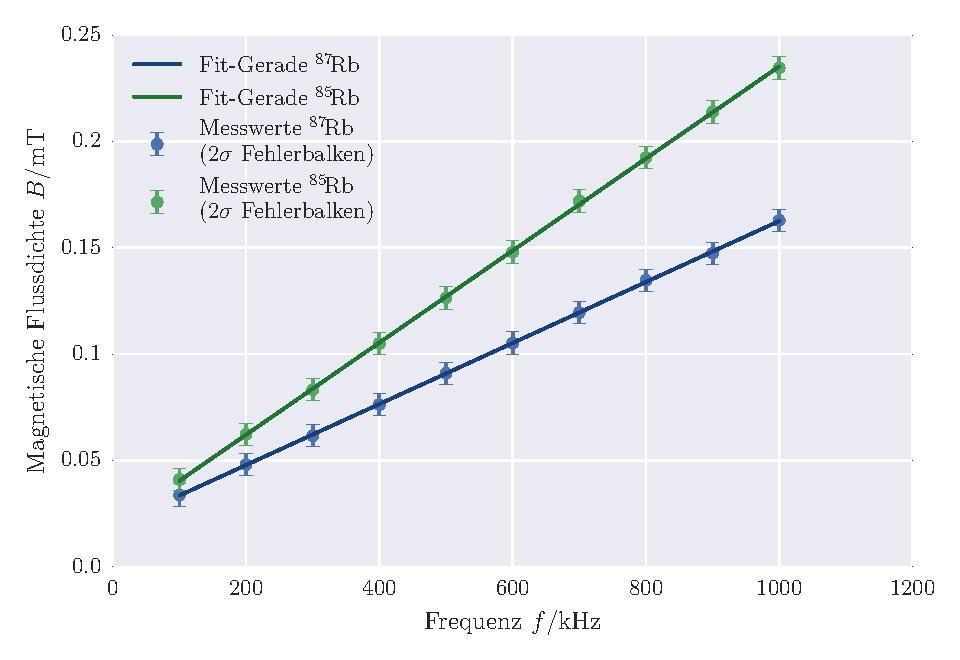
\includegraphics[scale=0.85]{../Grafiken/Resonanzstellen.pdf}
\caption{Darstellung der berechneten Magnetfelder für beide Isotope in Abhängigkeit der 
	jeweils eingestellten Frequenz. Die Fehlerbalken der Messwerte wurden verdoppelt um sichtbar zu sein.
	Neben den Messwerten sind auch die Ausgleichs-Geraden für beide Isotope dargestellt. \label{fig:resonanzstellen}}
\end{figure}
\FloatBarrier